%
\hsection{Downloading the Example Codes}%
\label{sec:downloadingExamples}%
%
\begin{figure}%
\centering%
%
\subfloat[][%
We use a web browser to visit the website~\expandafter\url{\databasesCodeRepo}. %
On the website, we click on the green \menu{Code} menu.%
\label{fig:examplesBrowser1website}%
]{\parbox[t]{0.9999\linewidth}{\centering\tightbox{%
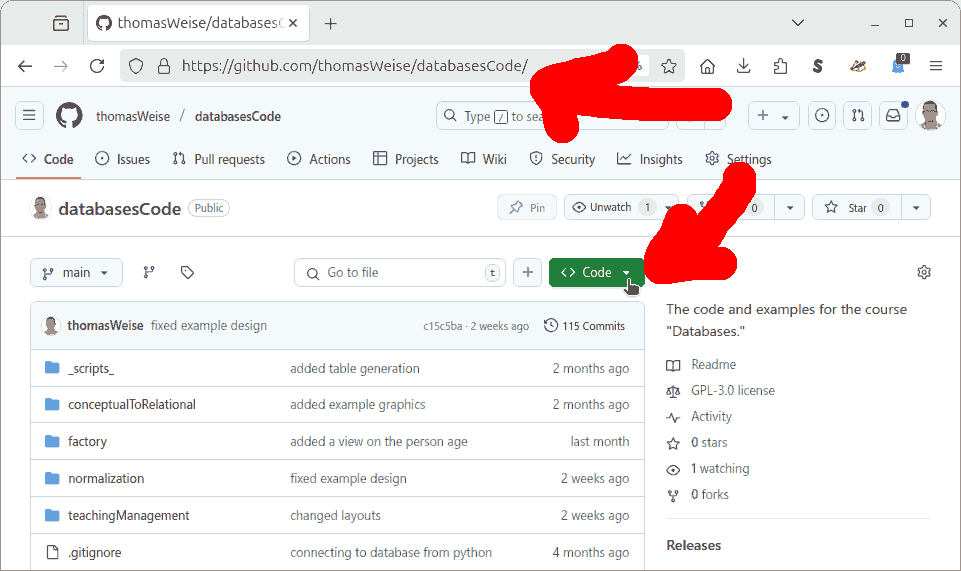
\includegraphics[width=0.7\linewidth]{\currentDir/examplesBrowser1website}}}}%
%
\floatRowSep%
%
\subfloat[][%
A small popup-menu appears, where we click on~\menu{Download ZIP}.%
\label{fig:examplesBrowser2beginDownload}%
]{\parbox[t]{0.9999\linewidth}{\centering\tightbox{%
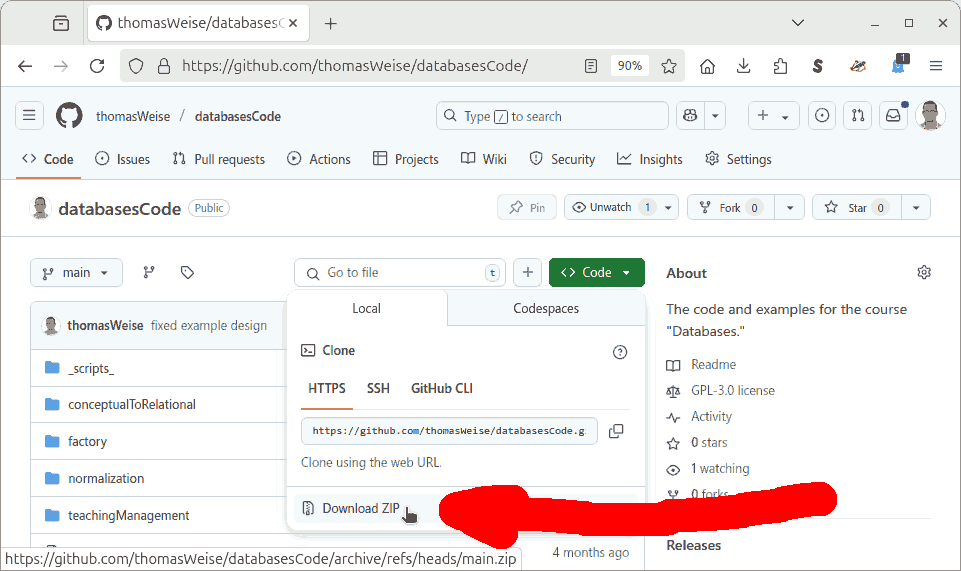
\includegraphics[width=0.7\linewidth]{\currentDir/examplesBrowser2beginDownload}}}}%
%
\label{fig:examplesBrowser:A}%
\caption{Downloading the examples from this book.}%
\end{figure}%
%
\begin{figure}%
\centering%
%
\subfloat[][%
Once the file is downloaded, we open it.%
\label{fig:examplesBrowser3downloaded}%
]{\parbox[t]{0.9999\linewidth}{\centering\tightbox{%
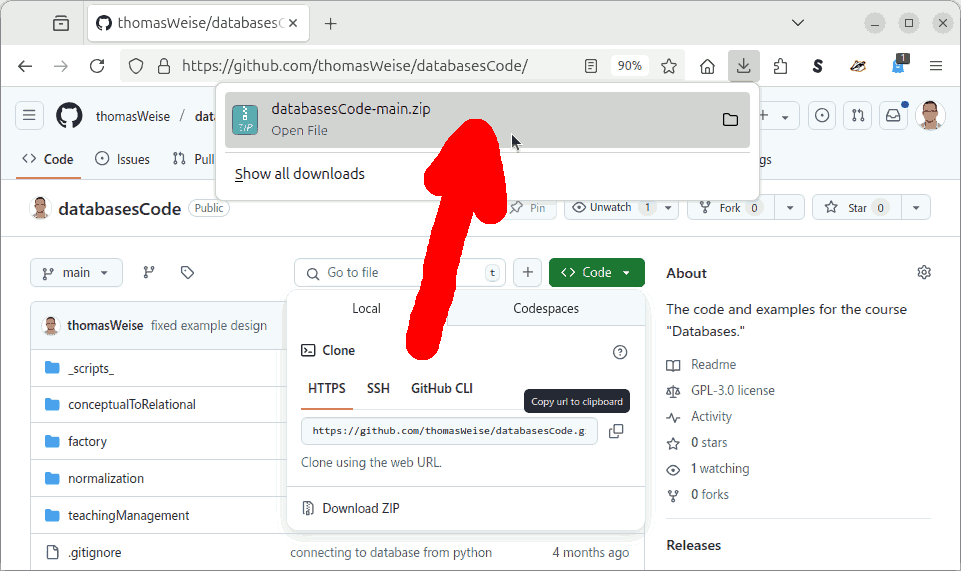
\includegraphics[width=0.7\linewidth]{\currentDir/examplesBrowser3downloaded}}}}%
%
\floatRowSep%
%
\subfloat[][%
In the opened archive, we can find \emph{all} the examples of this book. %
In folder \textil{factory}, we find the simple factory example.
\label{fig:examplesBrowser4opened}%
]{\parbox[t]{0.9999\linewidth}{\centering\tightbox{%
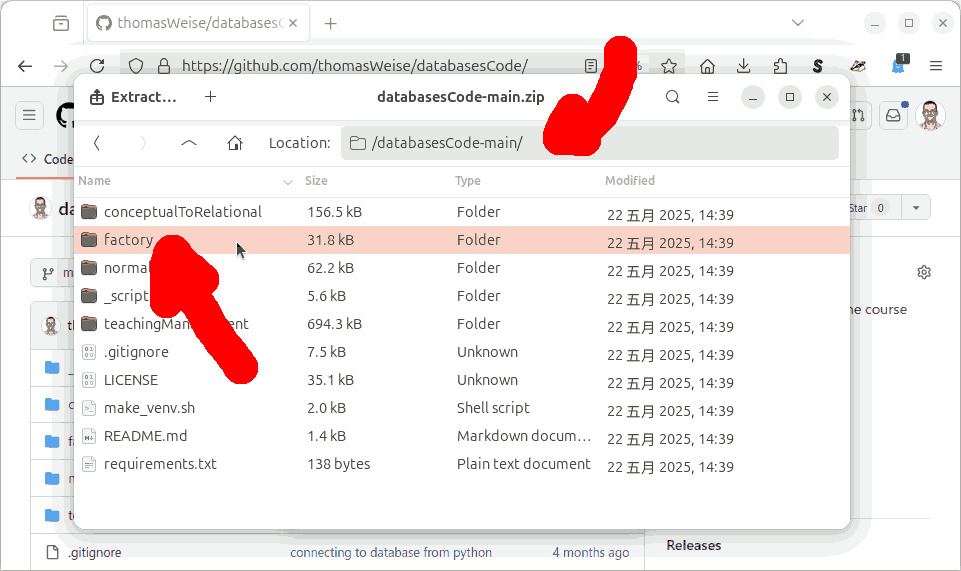
\includegraphics[width=0.7\linewidth]{\currentDir/examplesBrowser4opened}}}}%
%
\label{fig:examplesBrowser:B}%
\caption{Downloading the examples from this book.~(Continued)}%
\end{figure}%
%
In this book, we provide a lot of examples.
Some of them are \sql\ scripts that can be sent to the \postgresql\ \dbms\ \pgls{server} via the \psql~\pgls{client}.
Others are \pglspl{ERD} drawn with \yEd.
Yet others are domain-specific \db\ models developed with \pgmodeler.
For all examples, we always provide the source files.
So you do not need to type in the examples from the book.
You can download them!

All these examples are provided in the repository~\texttt{\databasesCodeRepoName} on \github.
There are two basic ways to obtain all of these examples:
First, you can download them using your web browser.
This basically requires no prerequisites except a web browser, which is usually part of any \pgls{OS}.
Second, you can use \pycharm\ \pgls{ide} to clone the \git\ repository and setting up \python\ dependencies in one swoop.
We discuss this option in \cref{sec:cloningExamplesRepoAndInstallingPsycopgUnderPyCharm}.
This, however, requires you to also first instally \python\ and \pycharm, which is discussed in our freely available sister course \citetitle{programmingWithPython}~\cite{programmingWithPython}.
If you have these tools available, then that might be the even more convenient choice.

For downloading the examples directly, you would visit this repository at \expandafter\url{\databasesCodeRepo}.
This is illustrated in \cref{fig:examplesBrowser:A}.
As shown in \cref{fig:examplesBrowser1website}, you would use your web browser to visit the website~\expandafter\url{\databasesCodeRepo}.
Once the website has loaded, you click on the green \menu{Code} menu.
Then, in \cref{fig:examplesBrowser2beginDownload}, a small popup-menu appears, where you click on~\menu{Download ZIP}.
This will download a so-called ZIP-archive, i.e., a file that contains a compressed folder structure with all files in our examples repository.
After the download completes, as illustrated in \cref{fig:examplesBrowser3downloaded}, you then can open the archive.
In the opened archive, you can find \emph{all} the examples of this book in a folder called \textil{databasesCode-main}.
This folder contains another folder called \textil{factory}, where you can find all the files belonging to our present example, as shown in \cref{fig:examplesBrowser4opened}.

Additionally, each source code listing has a headline containing some text like~\inQuotes{(stored in file \textil{myfile};.}
\textil{myfile} then is a clickable link that would take you directly to the file on \github.%
%
\FloatBarrier%
\endhsection%
%
